\documentclass[11pt]{article}
\usepackage[a4paper,margin=2.5cm]{geometry}
\usepackage[T1]{fontenc}
\usepackage[utf8]{inputenc}
\usepackage{amsmath,amssymb}
\usepackage{booktabs,array}
\usepackage{graphicx}
\usepackage{xcolor}
\usepackage[numbers,sort&compress]{natbib}
\usepackage[colorlinks=true,linkcolor=blue!50!black,citecolor=blue!50!black,urlcolor=blue!50!black]{hyperref}
\graphicspath{{../../examples/}}

\newcommand{\qgZ}{qg_Z}
\newcommand{\qgX}{qg_X}
\newcommand{\qgY}{qg_Y}

\title{What the polar bias can and cannot do for cryptography:\\
telling drift from eavesdropping in BB84, and certified quantum randomness}
\author{Vicente Humberto Monteverde\\
\small Universidad del Museo Social Argentino (UMSA), Argentina\\
\small ORCID 0000-0001-8884-4811}
\date{\small Draft of 26 September 2026}

\begin{document}
\maketitle

\begin{abstract}
We ask where the qg description of a qubit, $\qgZ=\langle\sigma_z\rangle$ and its companions
$\qgX,\qgY$~\cite{monteverde2026qang}, is useful for cryptography. Post-quantum cryptography
(lattice-based key encapsulation such as ML-KEM~\cite{fips203}) is classical and has no place for
it. Quantum cryptography does, because its raw data are qg values. (i) In BB84~\cite{bennett1984}
over a qubit channel with relaxation, the sum $A_Z=qg(0)+qg(1)$ of the received polar biases is a T1
witness. Natural relaxation raises it, while intercept-resend adds symmetric errors that leave it
unchanged. A likelihood-ratio monitor built on it detects intercept-resend as well as the standard
QBER monitor, but raises no false alarms when the memory's T1 degrades, where the QBER monitor fires in
48--100\% of windows. By construction it misses an attacker who mimics T1, which the QBER monitor
catches, so the two are complementary and neither changes the secret-key rate. (ii) For a qubit
random-number generator with a trusted measurement, the certified min-entropy is
$H_{\min}(Z|E)=-\log_2\big[(1+\sqrt{1-\qgX^2-\qgY^2})/2\big]$, independent of $\qgZ$. The usual
output-bias estimate is unsafe whenever the state is mixed: it certifies 0.97 bits per shot where
0.015 are private. A qg estimate from $\pm$-rotation test rounds is safe in every run, and a readout
calibration recovers 10--50\% more certified bits. On IonQ trapped-ion noise models, with an
environment ion that learns the output, the naive estimate stays near 1 bit while the qg estimate
remains safe and captures 82--90\% of the private randomness. All results are simulations, reproduced by scripts
and pinned by regression tests.
\end{abstract}

\section{Where qg does not apply: post-quantum cryptography}

Post-quantum schemes such as ML-KEM (Kyber)~\cite{fips203} or lattice and hash-based signatures run on
classical computers and are designed to resist quantum attacks. They involve no qubits and no
measurement statistics, so a coordinate for qubit measurements has nothing to contribute. The threat
they answer, Shor's algorithm, does not benefit from qg either; the project's reference notebook
documents it as a non-application. We state this first so that the rest is not read as a claim about
post-quantum security.

\section{BB84: drift or eavesdropper?}\label{sec:bb84}

\paragraph{Setting.} Alice sends $|0\rangle,|1\rangle$ (Z basis) or $|\pm\rangle$ (X basis); the
qubit waits in a memory or channel with amplitude damping $\gamma$ (T1) and dephasing $p$; Bob
measures with an asymmetric detector ($e_{01}=0.005$, $e_{10}=0.01$). This fits matter-qubit links
and on-chip demonstrations, not photon-polarization links, whose noise is mostly unital. Each sent
state gives one qg value at Bob,
\begin{equation}
qg(0)=1-2e(0\!\to\!1),\quad qg(1)=-1+2e(1\!\to\!0),\quad
A_Z=qg(0)+qg(1)=2\,[e(1\!\to\!0)-e(0\!\to\!1)],
\end{equation}
and likewise in X. $A_Z$ is the register-mean T1 witness of the companion paper~\cite{monteverde2026witness}:
relaxation creates only $1\to0$ errors and raises it, while intercept-resend on a fraction $f$ of the
qubits adds $f/4$ errors in every category and leaves it unchanged. The baseline channel has
$\gamma_0=0.02$, $p_0=0.01$.

\paragraph{Monitors.} Windows of $N$ compared bits, 1\% false alarms on the baseline. The
\emph{QBER monitor} tests the total error count. The \emph{qg monitor} is a generalized likelihood
ratio on the four error counts, in which ``attack'' ($f>0$) must beat both ``baseline'' and ``T1
drift'' ($\gamma$ free).

\begin{table}[t]
\centering\small
\caption{Alarm rates (1000 windows of $N=2000$ compared bits). The last column is the Shor--Preskill
secret fraction $1-h(Q_Z)-h(Q_X)$~\cite{shorpreskill2000}.}
\label{tab:bb84}
\begin{tabular}{lccc}
\toprule
scenario & QBER monitor & qg monitor & secret fraction\\
\midrule
baseline & 0.007 & 0.006 & 0.720\\
T1 drift, $\gamma$ $0.02\to0.04$ & 0.478 & \textbf{0.009} & 0.640\\
T1 drift, $\gamma$ $0.02\to0.06$ & 0.962 & \textbf{0.006} & 0.567\\
intercept-resend, $f=0.02$ & 0.218 & 0.271 & 0.668\\
intercept-resend, $f=0.05$ & 0.861 & 0.823 & 0.594\\
intercept-resend, $f=0.10$ & 1.000 & 0.994 & 0.481\\
T1-mimicking attack (extra $\gamma=0.04$) & \textbf{0.962} & 0.006 & 0.567\\
\bottomrule
\end{tabular}
\end{table}

\begin{figure}[t]
\centering
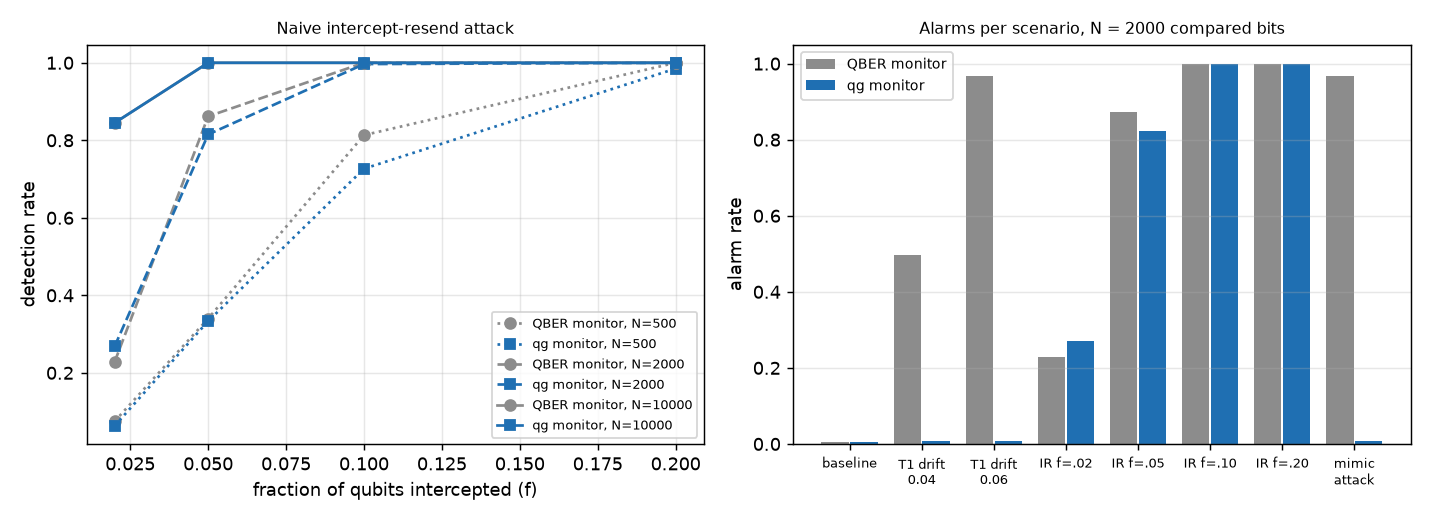
\includegraphics[width=\linewidth]{bb84_qg_eve_vs_noise.png}
\caption{Left: detection of intercept-resend vs the intercepted fraction, for $N=500$, 2000 and
10{,}000 compared bits. Right: alarm rates per scenario at $N=2000$.}
\label{fig:bb84}
\end{figure}

\paragraph{Results} (Table~\ref{tab:bb84}, Fig.~\ref{fig:bb84}).
\begin{itemize}
\item \emph{Equal detection, fewer false alarms.} The qg monitor detects intercept-resend as well
as the QBER monitor at every $N$ and $f$, but stays quiet when T1 degrades. The QBER monitor fires in
48--100\% of those windows.
\item \emph{The price, by design.} An attacker who couples the qubit to her ancilla through an
amplitude-damping interaction is, from Bob's side, identical to T1 drift. The qg monitor misses her
and the QBER monitor does not. Run together, QBER says that something changed and qg says what kind
of change it is.
\item \emph{No security gain.} The secret fraction falls in the same way in all cases. A security
proof must attribute every error to Eve~\cite{scarani2009}. The qg monitor is an operational
diagnostic.
\end{itemize}

\section{Certified random numbers}\label{sec:qrng}

A qubit QRNG~\cite{herrero2017} prepares $|+\rangle$ and measures Z. Dephasing and thermal
population leave the output unbiased, but then part of the randomness is classical noise that an
adversary holding the environment can know. With a trusted measurement and an adversary holding the
purification, her two conditional states are pure, with overlap $|\rho_{01}|=r_\perp/2$. By
Helstrom~\cite{helstrom1976} and the operational meaning of min-entropy~\cite{konig2009},
\begin{equation}\label{eq:hmin}
P_{\rm guess}(Z|E)=\frac{1+\sqrt{1-r_\perp^2}}{2},\qquad
H_{\min}(Z|E)=-\log_2P_{\rm guess},\qquad r_\perp=\sqrt{\qgX^2+\qgY^2}.
\end{equation}
The result is independent of $\qgZ$: only the coherence in the measured basis is private. For a pure
state it reduces to the classical $-\log_2\max(p_0,p_1)$. We checked Eq.~\eqref{eq:hmin} against an
explicit purification.

\paragraph{Estimators.} From $10^4$ test rounds per setting, with the readout
$\qgZ^{\rm meas}=a+b\,\qgZ$ ($e_{01}=0.015$, $e_{10}=0.04$) calibrated by the heralded sweep of the
companion paper. We compare four estimates. The \emph{naive} one is the output-bias estimate
$-\log_2\max(\hat p_0,\hat p_1)$. The \emph{qg one-sided} estimate takes $r_\perp$ from X and Y test
rounds with a single rotation each. The \emph{qg $\pm$} estimate measures each axis with both
rotations, so the offset $a$ cancels. The \emph{qg calibrated} estimate is the $\pm$ one divided by the
calibrated $b$. All qg estimates use a $3\sigma$ lower bound on $r_\perp$.

\begin{table}[t]
\centering\small
\caption{Certified bits per shot: mean estimate and, in parentheses, the fraction of runs above the
truth (unsafe). 300 repetitions.}
\label{tab:qrng}
\begin{tabular}{lcccc}
\toprule
scenario & truth & naive & qg $\pm$ & qg calibrated\\
\midrule
ideal $|+\rangle$ & 1.000 & 0.965 (0) & 0.512 (0) & 0.681 (0)\\
T2, $V=0.8$ & 0.322 & 0.964 (\textbf{1.00}) & 0.245 (0) & \textbf{0.286} (0)\\
T2, $V=0.5$ & 0.100 & 0.965 (\textbf{1.00}) & 0.077 (0) & \textbf{0.087} (0)\\
T2, $V=0.2$ & 0.015 & 0.965 (\textbf{1.00}) & 0.009 (0) & \textbf{0.010} (0)\\
thermal $p=0.05$, $V=0.9$ & 0.334 & 0.965 (\textbf{1.00}) & 0.254 (0) & \textbf{0.297} (0)\\
$e_{10}=0.10$, $V=0.95$ & 0.608 & 0.876 (\textbf{1.00}) & 0.341 (0) & \textbf{0.513} (0)\\
\bottomrule
\end{tabular}
\end{table}

\begin{figure}[t]
\centering
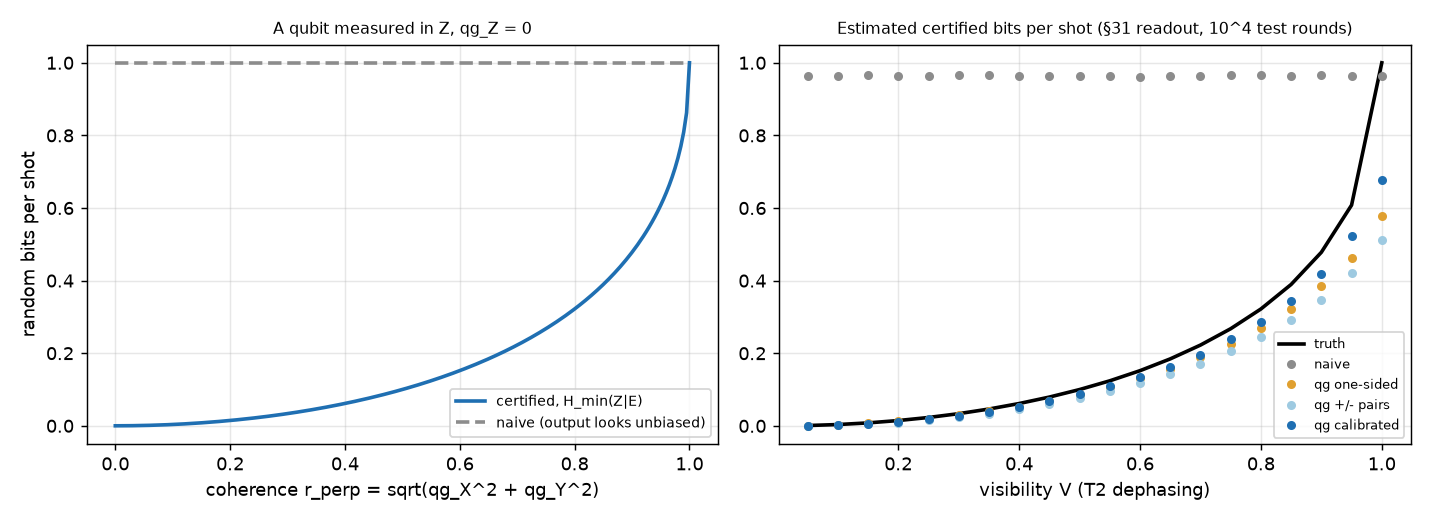
\includegraphics[width=\linewidth]{qrng_qg_certified.png}
\caption{Left: certified bits per shot vs the coherence $r_\perp$ at $\qgZ=0$, against the naive
reading. Right: estimates vs the visibility $V$.}
\label{fig:qrng}
\end{figure}

\paragraph{Results} (Table~\ref{tab:qrng}, Fig.~\ref{fig:qrng}).
\begin{itemize}
\item \emph{The output-bias estimate is unsafe} whenever the state is mixed: it overestimates in
every run.
\item \emph{The qg estimate is safe in every run} when each axis is measured with both rotations.
With a single rotation the readout offset inflates $r_\perp$, and at $V=0.2$ the estimate exceeds the
truth in 7\% of runs.
\item \emph{Calibration pays.} Dividing by the calibrated $b$ recovers 10--50\% more certified bits.
\item \emph{A near-perfect source is shot-hungry to certify.} $H_{\min}$ has an infinite slope at
$r_\perp=1$, the qg pole, so the $3\sigma$ bound gives 0.68, 0.81 and 0.89 bits per shot with
$10^4$, $10^5$ and $10^6$ test rounds.
\end{itemize}

\paragraph{On a trapped-ion noise model.} We ran the certifier on IonQ's cloud simulator with the
aria-1 and forte-1 noise models (free; nothing sent to a QPU), with a leak the adversary really holds.
A source ion starts in $|0\rangle$ and is read in X; a second ion, the environment, learns the X
value through a partial M{\o}lmer--S{\o}rensen gate $\mathrm{MS}(0,0,\theta)$. The output stays a fair
coin, while $H_{\min}(X|E)$ falls as in Eq.~\eqref{eq:hmin} with $r=|\cos2\pi\theta|$ (X and Z
exchanged). All circuits use native gates, so the service cannot merge rotations; each setting has
$10^4$ samples, three repetitions per model (Table~\ref{tab:qrngionq}). The naive estimate stays at
0.97--1.00 bits and overestimates in every run with a leak (four times the truth at $\theta=0.12$).
The qg $\pm$ estimate is safe in all 24 cells and captures 82--90\% of the truth with a leak. The
simulator's readout is almost perfect ($b\ge0.9998$), so calibration adds nothing there: the gain of
Table~\ref{tab:qrng} needs hardware-like readout errors and remains to be checked on a device. The
measured $r$ sits 1--1.5\% below the ideal, which is the MS gate error, correctly counted as lost
privacy.

\begin{table}[t]
\centering\small
\caption{Certified bits per shot on IonQ noise models (mean of 3 runs; aria-1 / forte-1 where they
differ). No qg estimate exceeds the truth in any run.}
\label{tab:qrngionq}
\begin{tabular}{lcccc}
\toprule
$\theta$ (turns) & truth & naive & qg one-sided & qg $\pm$\\
\midrule
0 (no leak) & 1.000 & 0.98 & 0.69 & 0.73\\
0.04 & 0.680 & 0.99 (\textbf{unsafe}) & 0.53 & \textbf{0.56 / 0.55}\\
0.08 & 0.433 & 0.98 / 0.97 (\textbf{unsafe}) & 0.37 / 0.36 & \textbf{0.38 / 0.37}\\
0.12 & 0.248 & 0.99 (\textbf{unsafe}) & 0.22 / 0.21 & \textbf{0.22}\\
\bottomrule
\end{tabular}
\end{table}

\section{Limitations}

(i) Everything is simulation: single-qubit models with i.i.d.\ rounds, and vendor noise models on IonQ's simulator, not hardware. (ii) The QRNG is
device-dependent (trusted measurement), not device-independent. (iii) Eq.~\eqref{eq:hmin} and the
BB84 security bound are standard results; qg writes them in measured quantities. (iv) The BB84
monitor is a diagnostic: an attacker who mimics relaxation is invisible to it, and the key rate is
unchanged. (v) The BB84 setting needs a relaxation mechanism (matter qubits); it does not describe
photon-polarization links.

\section{Code availability}
\sloppy
\texttt{examples/bb84\_qg\_eve\_vs\_noise.py} and \texttt{examples/qrng\_qg\_certified.py} and \texttt{examples/ionq\_sim\_qrng.py} in
\url{https://github.com/Viny2030/qang} (MIT license), with regression tests. Sections 40--42 of
\texttt{RESEARCH\_NOTES.md} give more detail, and \texttt{notebooks/qang\_criptografia\_colab.ipynb}
reproduces fast versions in Colab.

\section*{Acknowledgments and use of AI tools}
Generative AI tools (Anthropic Claude Opus 5.5) assisted with code, numerical experiments, tests and
drafting. The author framed the questions, made the design decisions, and reviewed and validated all
AI-assisted output, including every number reported here.

\bibliographystyle{unsrtnat}
\bibliography{../refs}
\end{document}
